\documentclass[11pt]{article}
\usepackage{myz310e-notes}
\hypersetup{pdftitle={Generative classifiers: the Bayes classifier and naive Bayes},pdfauthor={Emre Onur Kahya},pdfsubject={MYZ 310E Machine Learning in Physics, Fall 2026, lecture note 6 (week 4)}}
\newcommand{\w}{\vect{w}}
\usepackage{needspace}

\begin{document}
\NoteTitle{6}{4}{Generative classifiers: the Bayes\\ classifier and naive Bayes}{Generative classifiers}{%
A classifier can be built from density estimators: model how the data of each class are distributed, then let
Bayes' rule turn those densities into class probabilities. This note develops that recipe step by step and computes
it by hand on small tables; shows why the prior matters so much for rare classes; derives the quadratic and linear
decision boundaries produced by Gaussian class densities; works through the three common forms of naive Bayes
(binary, count and real-valued features), with and without smoothing; gives pseudocode and running times for every
algorithm; and compares the generative route with the discriminative one taken in Note~9. The same reasoning
underlies the likelihood-ratio tests of experimental physics and the use of today's generative models as
classifiers.}

\section{From scores to decisions}\label{sec:scores}

Note~1, Section~4, showed that the fewest errors are made by predicting, for every input, the class that is most
probable given that input. Practical classifiers reach this decision in two stages: they compute numbers that measure
how strongly $\x$ points to each class (a \emph{discriminant function} or \emph{score}), and then turn the numbers
into a choice. A trigger built on a neural network is a typical case: the network maps the detector hits of an event
to one number $g(\x)$, and the event is kept if $g(\x)$ exceeds a cut $\tau$. If $g(\x)$ estimates
$P(Y = 1 \mid \x)$, the cut $\tau = \tfrac12$ keeps exactly the events in which signal is more probable than
background; other cuts trade signal efficiency (the fraction of signal events kept) against purity (the fraction of
kept events that are signal), Section~\ref{sec:costs}. With $m$ classes there is one score
$g_c(\x)$ per class and the largest one wins; for two classes only the difference $g_1 - g_0$ matters, so a single
score and a cut describe the same rule. (From Section~\ref{sec:logspace} on, the scores are logarithms and are called
$s_c$.) Where do good scores come from? A \emph{generative} classifier
obtains them as class probabilities by modelling how the inputs of each class are distributed and applying Bayes'
rule; Section~\ref{sec:gendisc} compares it with the discriminative route.

\section{The Bayes classifier}\label{sec:bayes}

\subsection{Bayes' rule for classification}

As in Note~1, Section~2, the examples are i.i.d.\ draws of a pair $(\X, Y)$ from a distribution that is \emph{unknown}
and can only be estimated from the training set. The input is itself a vector of $d$ scalar random variables, so the
object of interest is the joint law of $d + 1$ variables, $P(\X, Y) = P(X_1, \dots, X_d, Y)$; Section~\ref{sec:naive}
will exploit this structure. The probability tools used below --- discrete and continuous variables, joint, marginal and
conditional distributions, Bayes' rule and independence --- are those of Note~2, Section~1, whose kaon-tagging example is
a one-feature preview of this note. Write
$p(\x, c)$ for the joint distribution: a density in $\x$ (a probability if $\x$ is discrete) and a probability in $c$.
The product rule (Note~2, Section~1.1) factorises it in two ways,
\[
  p(\x, c) = P(Y = c \mid \X = \x)\, p(\x) = p(\x \mid Y = c)\, P(Y = c) ,
\]
where $p(\x)$ is the marginal density of the inputs. Dividing by $p(\x)$ and writing the marginal as a sum over
classes (the law of total probability, $p(\x) = \sum_{c'} p(\x, c')$) gives Bayes' rule in the form used for
classification:
\begin{equation}\label{eq:bayes}
  \underbrace{P(Y = c \mid \X = \x)}_{\text{posterior}}
  = \frac{\overbrace{p(\x \mid Y = c)}^{\text{likelihood}}\; \overbrace{P(Y = c)}^{\text{prior}}}
         {\sum_{c'=1}^{m} p(\x \mid Y = c')\, P(Y = c')} .
\end{equation}
The \emph{class-conditional density} or \emph{likelihood} $p(\x \mid Y = c)$ says what examples of class $c$ look
like; the \emph{prior} $P(Y = c)$ says how common the class is before $\x$ is seen; the \emph{posterior} combines the
two. For discrete $\x$ the likelihood is a probability, for continuous $\x$ a density; the formula is the same.

\paragraph{Notation} $P_c = P(Y = c)$ is the prior and $p_c(\x) = p(\x \mid Y = c)$ the class density; hats mark
estimates from the training set ($\hat P_c$, $\hat p_c$); $s_c(\x)$ is the log-score of Section~\ref{sec:logspace}.
Classes are labelled $1, \dots, m$ in general and $0, 1$ when there are only two.

The \emph{Bayes classifier} estimates the likelihoods and the priors from the training set and plugs the estimates
into \eqref{eq:bayes}: (1)~split $\Dtrain$ by class into subsets of sizes $n_1, \dots, n_m$, with $\sum_c n_c = n$;
(2)~fit a density estimator $\hat p_c(\x)$ to each subset; (3)~estimate priors by class frequencies,
$\hat P_c = n_c / n$; (4)~predict $f(\x) = \argmax_c \hat p_c(\x)\, \hat P_c$, or report the normalised posteriors.
A word on the name: Note~1, Section~4, called $\argmax_c P(Y = c \mid \x)$ computed with the \emph{true} distribution
the Bayes classifier, and its error the Bayes error. The true distribution is never available, so the recipe above is
strictly a \emph{plug-in} estimate of that ideal rule; its expected error is never below the Bayes error, and
equals it only if the estimated densities and priors are exact. Following common usage we still call the recipe ``the
Bayes classifier'', and keep ``Bayes error'' for the error of the ideal rule.
The denominator of \eqref{eq:bayes} is the same for every class, so it matters only when probabilities, not just
decisions, are needed. Any density estimator can be used in step~2 --- a Gaussian (Note~2, Section~6), a histogram
(Note~3, Section~1), a kernel density estimate (Note~5, Section~4) or a deep generative model --- and the classifier
inherits its capacity and its weaknesses. With kernel density estimates the Bayes classifier is close to the
Parzen-window classifier of Note~5, Section~3; with $d$ large, it inherits the curse of dimensionality of Note~3,
Section~3. Equivalently, the class probabilities are the normalised joint probabilities $p(\x, c)$; in the
electron/pion example below the joint is simply a cell count divided by $n$ (reading~(i)), and Section~\ref{sec:gendisc}
returns to this view.

\subsection{Why the recipe is maximum likelihood}

Steps~1--3 are not ad hoc: they are what maximum likelihood (Note~2, Section~2) prescribes for the joint model
$p(\x, y) = p_{\theta_y}(\x \mid y)\, P_y$. The log-likelihood of the training set is
\[
  \ell = \sum_{i=1}^n \log\big[p_{\theta_{y_i}}(\x_i \mid y_i)\, P_{y_i}\big]
  = \sum_{c=1}^m \Big[\sum_{i:\, y_i = c} \log p_{\theta_c}(\x_i \mid c)\Big] + \sum_{c=1}^m n_c \log P_c .
\]
The parameters $\theta_c$ of class $c$ appear only in the $c$-th bracket, so each class density is fitted on its own
examples (steps~1--2). The priors appear only in the last sum, which must be maximised under the constraint
$\sum_c P_c = 1$. With a Lagrange multiplier $\lambda$ (the same calculation as for a categorical distribution in
Note~2, Section~2.1),
\[
  \frac{\partial}{\partial P_c}\Big[\sum_{c'} n_{c'} \log P_{c'} - \lambda\Big(\sum_{c'} P_{c'} - 1\Big)\Big]
  = \frac{n_c}{P_c} - \lambda = 0
  \quad\Rightarrow\quad P_c = \frac{n_c}{\lambda} ;
\]
summing over $c$ gives $1 = n/\lambda$, so $\lambda = n$ and $\hat P_c = n_c / n$ (step~3). The class frequencies are the
maximum-likelihood priors --- which also means they are only as good as the assumption that the training set has the
same class balance as the data the classifier will meet (Section~\ref{sec:odds}).

\subsection{Computing in log space}\label{sec:logspace}

Densities in high dimension underflow (Note~2, Section~6): a product of 500 per-feature probabilities of order
$10^{-2}$ is $10^{-1000}$, far below the smallest positive normal double-precision number, about $10^{-308}$ (the
hardware can go down to about $10^{-324}$ only by giving up precision). Work instead with the
\emph{log-scores}
\[
  s_c(\x) = \log \hat p_c(\x) + \log \hat P_c .
\]
The decision is $\argmax_c s_c(\x)$, since the logarithm is increasing. The posteriors are the normalised
exponentials $\exp(s_c) / \sum_{c'} \exp(s_{c'})$, and these underflow again. The fix is to factor out the largest
term: with $s_{\max} = \max_c s_c$,
\[
  \log \sum_{c'} e^{s_{c'}} = s_{\max} + \log \sum_{c'} e^{s_{c'} - s_{\max}} ,
  \qquad
  \hat P(Y = c \mid \x) = \frac{e^{s_c - s_{\max}}}{\sum_{c'} e^{s_{c'} - s_{\max}}} .
\]
Every exponent is now $\le 0$ and at least one equals $0$, so the sum lies between $1$ and $m$ and nothing overflows or
underflows to a meaningless $0/0$. This is the log-sum-exp trick of Note~5, Section~3.3, applied to the log-scores;
the second formula is their softmax. Algorithm~\ref{alg:bayes} summarises the whole classifier.

\begin{algorithm}[tbp]
\caption{Generic Bayes classifier (any density estimator)}\label{alg:bayes}
\footnotesize
\begin{algorithmic}[1]
\Require training set $\{(\x_i, y_i)\}_{i=1}^n$ with $y_i \in \{1, \dots, m\}$; a density-fitting routine \textsc{FitDensity}
\Function{Fit}{$\Dtrain$}
  \For{$c = 1, \dots, m$}
    \State $D_c \gets \{\x_i : y_i = c\}$, \quad $n_c \gets |D_c|$ \Comment{split by class}
    \State $\hat P_c \gets n_c / n$ \Comment{maximum-likelihood prior}
    \State $\hat p_c \gets \Call{FitDensity}{D_c}$ \Comment{e.g.\ Gaussian, histogram, KDE}
  \EndFor
\EndFunction
\Function{Predict}{$\x$}
  \For{$c = 1, \dots, m$}
    \State $s_c \gets \log \hat p_c(\x) + \log \hat P_c$ \Comment{log-score; never form $\hat p_c(\x)$ itself}
  \EndFor
  \State $s_{\max} \gets \max_c s_c$; \quad $Z \gets s_{\max} + \log \sum_{c} \exp(s_c - s_{\max})$ \Comment{log-sum-exp $= \log \hat p(\x)$}
  \State $r_c \gets \exp(s_c - Z)$ for every $c$ \Comment{posteriors $\hat P(c \mid \x)$, sum to one}
  \State \Return $\hat y = \argmax_c s_c$ and $(r_1, \dots, r_m)$
\EndFunction
\end{algorithmic}
\end{algorithm}

\begin{runtime}{generic Bayes classifier}
Let $t_{\mathrm{fit}}(n_c)$ and $t_{\mathrm{eval}}$ be the costs of fitting one class density and evaluating it once.
\emph{Training}: $O(n)$ to split the data by label (one pass) plus $\sum_c t_{\mathrm{fit}}(n_c)$.
\emph{Prediction per query}: $m\, t_{\mathrm{eval}}$ for the log-scores plus $O(m)$ for the maximum and the log-sum-exp.
\emph{Memory}: whatever the $m$ estimators store. The costs therefore come from the density estimator: a parametric
density (Gaussian, naive Bayes) stores a fixed number of parameters and evaluates in time independent of $n$, whereas a
kernel density estimate stores all $n$ examples, $O(nd)$ memory, and costs $O(nd)$ per query (Note~5) --- the price of
a non-parametric model; a batch of $q$ queries is one $O(qnd)$ distance computation, fast on a GPU but still linear in $n$.
\end{runtime}

\subsection{A first example with discrete features}

When the features take a few discrete values, the class-conditional distributions can be estimated by counting, and
the whole classifier can be computed by hand.

\needspace{16\baselineskip}
\begin{worked}{particle identification from a count table}
A detector must distinguish electrons from charged pions with two coarse observables: whether a threshold Cherenkov
counter fired (C $\in$ \{yes, no\}) and whether the ratio of calorimeter energy to track momentum is close to one
($E/p \in$ \{high, low\}). Electrons tend to fire the counter and deposit all their energy; pions mostly do not. A
calibration sample of $n = 200$ identified particles gives the counts in the first two numerical columns below; the
other columns are computed from them. The column $\Lambda(\x) = \hat P(\x \mid e) / \hat P(\x \mid \pi)$ is the
\emph{likelihood ratio}: how many times more typical the observation is of electrons than of pions. $\Lambda > 1$ means
that the observation alone favours electrons (Section~\ref{sec:odds} develops this).

\begin{center}\footnotesize
\setlength{\tabcolsep}{4.5pt}
\begin{tabular}{@{}llrrccccccc@{}}\toprule
C & $E/p$ & electrons & pions & $\hat P(\x \mid e)$ & $\hat P(\x \mid \pi)$ & $\Lambda(\x)$ & $\hat P_e \hat P(\x \mid e)$ &
$\hat P_\pi \hat P(\x \mid \pi)$ & $\hat P(e \mid \x)$ & decision \\ \midrule
yes & high & 28 & 8 & 0.70 & 0.05 & 14 & 0.14 & 0.04 & $7/9 = 0.78$ & $e$ \\
yes & low & 6 & 16 & 0.15 & 0.10 & 1.5 & 0.03 & 0.08 & $3/11 = 0.27$ & $\pi$ \\
no & high & 4 & 24 & 0.10 & 0.15 & 0.67 & 0.02 & 0.12 & $1/7 = 0.14$ & $\pi$ \\
no & low & 2 & 112 & 0.05 & 0.70 & 0.071 & 0.01 & 0.56 & $1/57 = 0.018$ & $\pi$ \\ \midrule
\multicolumn{2}{@{}l}{total} & 40 & 160 & 1 & 1 & & & & & \\ \bottomrule
\end{tabular}
\end{center}

\emph{Priors}: $\hat P_e = 40/200 = 0.2$ and $\hat P_\pi = 160/200 = 0.8$.
\emph{Likelihoods}: divide each count column by its total, e.g.\ $\hat P(\text{yes, high} \mid e) = 28/40 = 0.70$ and
$\hat P(\text{yes, high} \mid \pi) = 8/160 = 0.05$.
\emph{Posteriors}: multiply by the priors and normalise each row. For (yes, high): $0.70 \times 0.2 = 0.14$ and
$0.05 \times 0.8 = 0.04$, so $\hat P(e \mid \text{yes, high}) = 0.14/0.18 = 7/9 \approx 0.78$.

\emph{Reading the result.} (i) The products $\hat P_c \hat P(\x \mid c)$ are just the cell counts divided by $n$ (e.g.\
$28/200 = 0.14$), so the posterior is the fraction of electrons in the cell, $28/36$; with a histogram density the Bayes
classifier is the cell-majority vote of Note~3, Section~1. (ii) For (yes, low) the evidence favours electrons ($\Lambda = 1.5 > 1$),
yet the decision is pion: the prior odds $0.2/0.8$ outweigh it. With equal priors the posterior would be
$0.15/(0.15 + 0.10) = 0.6$ and the decision electron. (iii) The training error is $(6 + 4 + 2 + 8)/200 = 10\%$: the
electrons outside (yes, high) and the pions inside it.
\end{worked}

\subsection{Posterior odds, likelihood ratio and prior}\label{sec:odds}

For two classes, write \eqref{eq:bayes} for $c = 1$ and $c = 0$ and divide: the common denominator $p(\x)$ cancels,
\begin{equation}\label{eq:odds}
  \underbrace{\frac{P(Y = 1 \mid \x)}{P(Y = 0 \mid \x)}}_{\text{posterior odds}}
  = \underbrace{\frac{p(\x \mid Y = 1)}{p(\x \mid Y = 0)}}_{\text{likelihood ratio } \Lambda(\x)}
  \times \underbrace{\frac{P(Y = 1)}{P(Y = 0)}}_{\text{prior odds}} .
\end{equation}
Taking logarithms, \emph{log posterior odds = log-likelihood ratio + log prior odds}: the data enter only through
$\Lambda(\x)$, and the prior adds a constant. Since the posterior odds $o$ and the posterior probability are related by
$P(Y = 1 \mid \x) = o / (1 + o)$, the rule ``predict class 1 if its posterior exceeds $\tfrac12$'' is the rule
``predict class 1 if $\Lambda(\x) > P_0 / P_1$''. The prior shifts the threshold on the likelihood ratio.

Figure~\ref{fig:prior} shows two unit-variance Gaussian classes two and a half standard deviations apart, background at
$0$ and signal at $2.5$. Here $\log \Lambda(x) = -\tfrac12 (x - 2.5)^2 + \tfrac12 x^2 = 2.5\,x - 3.125$, so the
boundary $\log \Lambda(x) = \log(P_0/P_1)$ is at $x = \big(3.125 + \log(P_0/P_1)\big)/2.5$. With equal priors it sits
half-way, at $x = 1.25$; if the signal makes up 1\% of the data, $\log 99 = 4.595$ moves it to $x \approx 3.09$, and
most of the signal is classified as background. This is correct --- it minimises the number of errors --- but it may not
be what we want, which is why decisions with unequal costs move the threshold again (Section~\ref{sec:costs}). Because
the two factors separate, a classifier trained with one class balance can be corrected for another by rescaling its
odds, provided the class-conditional densities are unchanged~\cite{saerens2002}: multiply the odds by
$(P_1^{\mathrm{new}}/P_0^{\mathrm{new}}) / (P_1^{\mathrm{old}}/P_0^{\mathrm{old}})$. For example, a classifier trained
on a balanced sample (prior odds $1$) outputs $0.8$ for an event, i.e.\ posterior odds $0.8/0.2 = 4$. In the real data
signal is $1\%$ of the events, prior odds $1/99$, so the corrected odds are $4 \times 1/99 = 0.0404$ and the corrected
posterior is $0.0404/1.0404 = 0.039$: a confident-looking $0.8$ becomes a $4\%$ chance. This is also why priors
estimated by counting the training set (Section~\ref{sec:bayes}) must be replaced when the training sample was
balanced by design.

\begin{figure}[htbp]
\centering
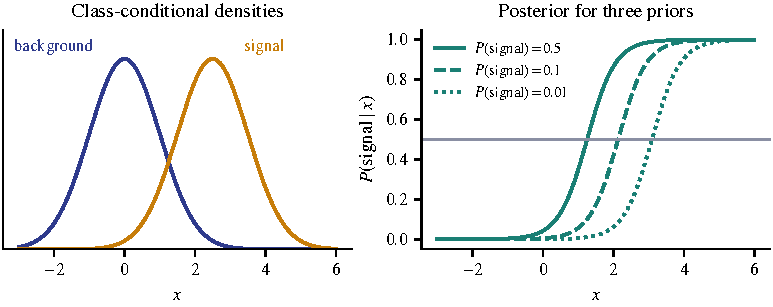
\includegraphics[width=0.9\linewidth]{figures/prior_shift.pdf}
\caption{The same class-conditional densities (left) give different posteriors (right) under different priors. The
decision boundary is where the posterior crosses $\tfrac12$: $x = 1.25$, $2.13$ and $3.09$ for signal fractions
$0.5$, $0.1$ and $0.01$.}
\label{fig:prior}
\end{figure}

\begin{worked}{a rare signal and a good trigger (posterior is not likelihood)}
A trigger accepts signal events with efficiency $P(\text{pass} \mid S) = 0.95$ and background events with
probability $P(\text{pass} \mid B) = 0.02$. Signal is one event in a thousand, $P(S) = 10^{-3}$. What fraction of the
accepted events is signal?

\emph{By counting.} Out of $10^6$ events, $1000$ are signal, of which $950$ pass; $999\,000$ are background, of which
$0.02 \times 999\,000 = 19\,980$ pass. The accepted sample contains $950$ signal events out of $20\,930$:
$P(S \mid \text{pass}) = 950 / 20\,930 = 0.045$.

\emph{By odds.} $\Lambda = 0.95/0.02 = 47.5$; prior odds $= 0.001/0.999 = 1.001 \times 10^{-3}$; posterior odds
$= 47.5 \times 1.001 \times 10^{-3} = 0.0475$, and $P(S \mid \text{pass}) = 0.0475/1.0475 = 0.045$.

The likelihood $P(\text{pass} \mid S) = 0.95$ and the posterior $P(S \mid \text{pass}) = 0.045$ differ by a factor of
twenty. Confusing them is the \emph{base-rate fallacy}; the same arithmetic explains why a positive result of a good
medical test for a rare disease is usually a false alarm. Now add a second selection with the same efficiencies, and
assume that once the class is fixed the two selections pass or fail independently:
$P(\text{both pass} \mid S) = 0.95^2$ and $P(\text{both pass} \mid B) = 0.02^2$. This is \emph{conditional independence},
$P(a, b \mid Y) = P(a \mid Y)\, P(b \mid Y)$; it does not make the two selections independent overall, since both pass
mostly on signal events. The combined likelihood ratio is $0.95^2/0.02^2 = 47.5^2$, so the odds are multiplied by $47.5$
once more: $0.0475 \times 47.5 = 2.26$, and $P(S \mid \text{both pass}) = 2.26/3.26 = 0.69$. Multiplying likelihood ratios of
several pieces of evidence is exactly what naive Bayes does (Section~\ref{sec:naive}) --- and it is correct only if the
pieces are conditionally independent.
\end{worked}

\subsection{Unequal costs}\label{sec:costs}

Suppose missing a signal event (predicting $0$ when $Y = 1$) costs $C_1$ and accepting a background event (predicting
$1$ when $Y = 0$) costs $C_0$, while correct decisions cost nothing. At a given $\x$ the expected cost of each
decision is
\[
  \E[\text{cost} \mid \text{predict } 1, \x] = C_0\, P(Y = 0 \mid \x), \qquad
  \E[\text{cost} \mid \text{predict } 0, \x] = C_1\, P(Y = 1 \mid \x) .
\]
Predict $1$ when the first is smaller: $C_1 P(Y = 1 \mid \x) > C_0 P(Y = 0 \mid \x)$. Dividing by
$C_1 P(Y = 0 \mid \x)$ and using \eqref{eq:odds} gives the first two forms below; for the third, write
$p = P(Y = 1 \mid \x)$ and $P(Y = 0 \mid \x) = 1 - p$, so that $C_1 p > C_0 (1 - p)$ becomes $p\,(C_0 + C_1) > C_0$:
\begin{equation}\label{eq:cost}
  \Lambda(\x)\,\frac{P_1}{P_0} > \frac{C_0}{C_1}
  \quad\Longleftrightarrow\quad
  \Lambda(\x) > \frac{C_0\, P_0}{C_1\, P_1}
  \quad\Longleftrightarrow\quad
  P(Y = 1 \mid \x) > \frac{C_0}{C_0 + C_1} .
\end{equation}
Equal costs give back the threshold $\tfrac12$. Costs and priors enter only through the product $C_1 P_1$ versus
$C_0 P_0$: making signal ten times more expensive to miss has the same effect as multiplying the prior odds
$P_1/P_0$ by ten. In Figure~\ref{fig:prior} with $P_1 = 0.01$ and $C_1 = 10\, C_0$, the threshold is
$\Lambda > 0.99/0.1 = 9.9$, i.e.\ $2.5\, x - 3.125 > \log 9.9 = 2.29$, so $x > 2.17$, between the error-minimising
boundaries for priors $0.01$ ($3.09$) and $0.5$ ($1.25$). For a rare signal, ten times larger odds is almost the same as
ten times larger $P_1$: $P_1 = 0.1$ gives the boundary $2.13$ instead of $2.17$, because raising $P_1$ also lowers $P_0$.

\begin{physics}{the Neyman--Pearson lemma and learned likelihood ratios}
In a search for a rare process the prior is tiny and largely unknown, so physicists rank events by the likelihood
ratio $\Lambda(\x)$ itself. The Neyman--Pearson lemma~\cite{neyman1933} states that, for two fully specified
(simple) hypotheses and any fixed rate of falsely accepted background, the test that accepts events with large
$\Lambda(\x)$ has the highest signal efficiency (efficiency and rejection as in Note~4, Section~2). Ranking by $\Lambda$ is not in conflict with ranking by the posterior:
for any fixed prior, the posterior odds are $\Lambda(\x)$ times a constant, so both orderings of the events are the
same. The advantage of $\Lambda$ is that it can be computed without knowing the prior; only the position of the cut
depends on the prior (and on the costs). The class densities are
rarely known in closed form, but a well-calibrated classifier trained on simulated signal and background events
estimates $P(Y = 1 \mid \x)$, and \eqref{eq:odds} turns it back into $\Lambda(\x)$: divide the posterior odds by the
prior odds of the training sample. This ``likelihood-ratio trick'' lets neural networks stand in for intractable
likelihoods in parameter inference~\cite{cranmer2015}.
\end{physics}

\section{Gaussian class densities}\label{sec:gaussian}

\subsection{Quadratic discriminant analysis}

Let each class be Gaussian, $p(\x \mid Y = c) = \Normal(\x; \vmu_c, \Sigma_c)$, with parameters fitted by the class
means and covariances (Note~2, Section~6). Taking the logarithm of the Gaussian density,
\[
  s_c(\x) = \log \Normal(\x; \vmu_c, \Sigma_c) + \log P_c
  = -\tfrac12 (\x - \vmu_c)\T \Sigma_c^{-1} (\x - \vmu_c) - \tfrac12 \log\lvert\Sigma_c\rvert + \log P_c
  - \tfrac{d}{2} \log 2\pi .
\]
The last term is common to all classes and can be dropped. Expand the quadratic form, using that $\Sigma_c^{-1}$ is
symmetric so that $\x\T \Sigma_c^{-1} \vmu_c = \vmu_c\T \Sigma_c^{-1} \x$:
\[
  (\x - \vmu_c)\T \Sigma_c^{-1} (\x - \vmu_c) = \x\T \Sigma_c^{-1} \x - 2\, \vmu_c\T \Sigma_c^{-1} \x
  + \vmu_c\T \Sigma_c^{-1} \vmu_c .
\]
Hence every log-score is a quadratic function of $\x$,
\begin{equation}\label{eq:qda}
  s_c(\x) = \underbrace{-\tfrac12\, \x\T \Sigma_c^{-1} \x}_{\text{quadratic}}
  + \underbrace{(\Sigma_c^{-1} \vmu_c)\T \x}_{\text{linear}}
  \underbrace{- \tfrac12\, \vmu_c\T \Sigma_c^{-1} \vmu_c - \tfrac12 \log\lvert\Sigma_c\rvert + \log P_c}_{\text{constant}} ,
\end{equation}
and so is the difference $s_1(\x) - s_0(\x)$. The boundary $s_1(\x) = s_0(\x)$ is a quadric: an ellipse, a parabola or a
hyperbola (or a pair of lines) in two dimensions. This is \emph{quadratic discriminant analysis} (QDA). Each term has a
meaning: the quadratic and linear terms, together with $-\tfrac12 \vmu_c\T \Sigma_c^{-1} \vmu_c$, make up minus half the
squared Mahalanobis distance to the class mean (Note~2, Section~4), the log-determinant
penalises broad classes (a broad density spreads its unit probability thinly, so near its centre it is lower than a
narrow one; far out in the tails it is higher, Section~\ref{sec:onedim}), and the log-prior favours common classes.

\subsection{One dimension: one threshold or two}\label{sec:onedim}

In one dimension, \eqref{eq:qda} reads $s_c(x) = -(x - \mu_c)^2 / (2\sigma_c^2) - \log \sigma_c + \log P_c$.

\emph{Equal variances.} With $\sigma_0 = \sigma_1 = \sigma$ the $\log\sigma$ terms cancel and, using
$(x - \mu_0)^2 - (x - \mu_1)^2 = (\mu_1 - \mu_0)(2x - \mu_0 - \mu_1)$,
\[
  s_1(x) - s_0(x) = \frac{(\mu_1 - \mu_0)(2x - \mu_0 - \mu_1)}{2\sigma^2} + \log\frac{P_1}{P_0} ,
\]
which is linear in $x$. Setting $s_1 - s_0 = 0$, moving the prior term to the right-hand side and multiplying by $2\sigma^2/(\mu_1 - \mu_0)$ gives
$2x - \mu_0 - \mu_1 = \big(2\sigma^2/(\mu_1 - \mu_0)\big) \log(P_0/P_1)$; dividing by $2$, the score difference
vanishes at the single threshold
\begin{equation}\label{eq:thr1d}
  x^* = \frac{\mu_0 + \mu_1}{2} + \frac{\sigma^2}{\mu_1 - \mu_0} \log\frac{P_0}{P_1} .
\end{equation}
The threshold sits at the midpoint, shifted away from the more probable class.

\emph{Unequal variances.} The $x^2$ terms no longer cancel, $s_1 - s_0 = 0$ is a quadratic equation, and there can be
two thresholds.

\begin{worked}{two Gaussian classes on a line}
(a) Class~0 is $\Normal(0, 1)$, class~1 is $\Normal(3, 1)$, and class~1 is rarer, $P_1 = 0.25$. By
\eqref{eq:thr1d}, $x^* = 1.5 + \tfrac13 \log 3 = 1.5 + 0.366 = 1.866$. Check: at $x = 1.866$ both
$P_c\, p(x \mid c)$ equal $0.0524$. The Bayes error follows by standardising (Note~2, Section~3.1), with $\Phi$ the
standard normal distribution function:
$0.75\, P(X > x^* \mid 0) + 0.25\, P(X < x^* \mid 1) = 0.75\,[1 - \Phi(1.866)] + 0.25\, \Phi(1.866 - 3)
= 0.75 \times 0.031 + 0.25 \times 0.128 = 0.023 + 0.032 = 5.5\%$.

(b) Class~0 is $\Normal(0, 1)$, class~1 is $\Normal(2, 2^2)$, equal priors. Then
\[
  s_1(x) - s_0(x) = -\frac{(x - 2)^2}{8} - \log 2 + \frac{x^2}{2} .
\]
Multiply by $8$: $-(x^2 - 4x + 4) - 8 \log 2 + 4x^2 = 3x^2 + 4x - (4 + 8\log 2) = 3x^2 + 4x - 9.545$. The roots are
\[
  x = \frac{-4 \pm \sqrt{16 + 12 \times 9.545}}{6} = \frac{-4 \pm 11.43}{6} ,
  \qquad x_- = -2.571, \quad x_+ = 1.238 .
\]
The leading coefficient is positive, so $s_1 > s_0$ outside the roots: predict class~0 for $-2.571 < x < 1.238$ and
class~1 on both sides. The narrow class owns an interval; the broad class wins in both tails, because far from both
means the narrow density decays faster. The Bayes error of this rule (built from the true densities) is $22.7\%$;
the best rule with a single threshold
(at $1.238$) has $23.0\%$, so here the far-left region matters little --- but it is there, and in higher dimensions the
same effect produces the closed boundary around a compact class in Figure~\ref{fig:bayesgauss}, centre.
Figure~\ref{fig:gauss1d} shows both cases.
\end{worked}

\begin{figure}[htbp]
\centering
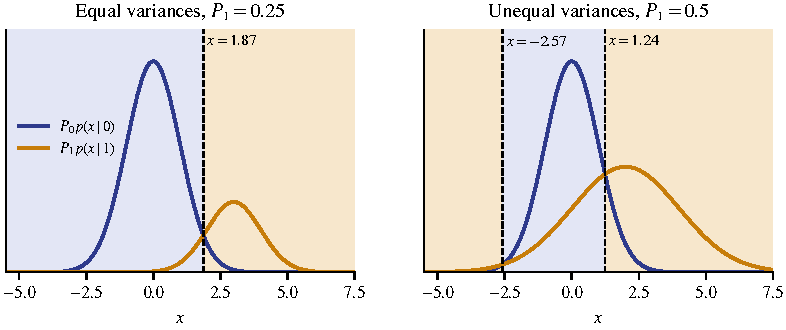
\includegraphics[width=0.9\linewidth]{figures/n6_gauss1d.pdf}
\caption{The two cases of the worked example. Curves are $P_c\, p(x \mid c)$; shading marks the predicted class
(indigo: class~0, amber: class~1). Left: equal variances give one threshold, shifted from the midpoint $1.5$ away from
the more probable class~0. Right: unequal variances give two thresholds; the narrow class~0 owns the interval between
them.}
\label{fig:gauss1d}
\end{figure}

\begin{worked}{a compact class in the plane}
In $d = 2$, class~0 is $\Normal(\vect{0}, I)$ and class~1 is the broader $\Normal(\vect{0}, 9I)$, with equal priors.
Write $r^2 = x_1^2 + x_2^2$. Since $\lvert 9I\rvert = 81$, $\tfrac12 \log\lvert 9I \rvert = \log 9$, and
\eqref{eq:qda} gives $s_0 = -r^2/2$ and $s_1 = -r^2/18 - \log 9$ (common terms dropped). Hence
\[
  s_1(\x) - s_0(\x) = \frac{r^2}{2} - \frac{r^2}{18} - \log 9 = \frac{4}{9}\, r^2 - \log 9 ,
\]
which vanishes on the circle $r^2 = \tfrac94 \log 9 = 4.94$, radius $r = 2.22$: class~0 inside, class~1 outside, a
closed QDA boundary with no linear part. For $\x = (1, 1)\T$, $r^2 = 2$ and $s_1 - s_0 = 0.889 - 2.197 = -1.31$, so
$P(Y = 1 \mid \x) = e^{s_1}/(e^{s_0} + e^{s_1}) = 1/(1 + e^{-(s_1 - s_0)}) = 1/(1 + e^{1.31}) = 0.21$: class~0. No
straight line can separate a disc from its surroundings, so LDA (next subsection) cannot represent this rule; here the
two means even coincide, so its weight vector is zero.
\end{worked}

\begin{figure}[tbp]
\centering
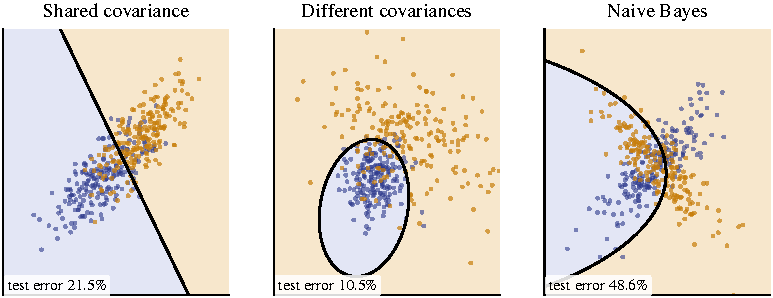
\includegraphics[width=\linewidth]{figures/bayes_gaussians.pdf}
\caption{Gaussian Bayes classifiers fitted to 200 points per class (indigo and amber), errors on $10^4$ fresh points.
Left: shared covariance gives a straight boundary. Centre: a compact class inside a broad one needs the quadratic
boundary of QDA. Right: the two classes have the same mean and variances and differ only in the sign of their
correlation; naive Bayes cannot see the difference.}
\label{fig:bayesgauss}
\end{figure}

\subsection{Shared covariance: linear discriminant analysis}

If all classes share one covariance $\Sigma$, the quadratic term $-\tfrac12 \x\T \Sigma^{-1} \x$ of \eqref{eq:qda} is
identical for every class and cancels in every comparison, and so does $-\tfrac12 \log\lvert\Sigma\rvert$. What remains
is a linear score per class,
\begin{equation}\label{eq:ldamulti}
  s_c(\x) = \w_c\T \x + b_c, \qquad \w_c = \Sigma^{-1} \vmu_c, \qquad b_c = -\tfrac12\, \vmu_c\T \Sigma^{-1} \vmu_c + \log P_c ,
\end{equation}
and for two classes the difference
\begin{equation}\label{eq:lda}
  s_1(\x) - s_0(\x) = \w\T\x + b, \qquad \w = \Sigma^{-1}(\vmu_1 - \vmu_0), \qquad
  b = -\tfrac12 \big(\vmu_1\T\Sigma^{-1}\vmu_1 - \vmu_0\T\Sigma^{-1}\vmu_0\big) + \log\frac{P_1}{P_0} .
\end{equation}
This is \emph{linear discriminant analysis} (LDA): the decision boundary is a hyperplane. Before expanding, the score
was $s_c(\x) = -\tfrac12 \Delta_c^2(\x) + \log P_c + \text{(terms common to all classes)}$, with
$\Delta_c^2(\x) = (\x - \vmu_c)\T \Sigma^{-1} (\x - \vmu_c)$ the squared Mahalanobis distance to $\vmu_c$ (Note~2,
Section~4). With equal priors the largest score therefore belongs to the smallest $\Delta_c$: the rule assigns $\x$ to
the class whose mean is nearest in Mahalanobis distance. If moreover $\Sigma = \sigma^2 I$, it assigns $\x$ to the
nearest mean in Euclidean distance --- the \emph{nearest-centroid} classifier, which Note~9, Section~2, studies as a
linear classifier in its own right. In practice $\Sigma$ is estimated by
pooling the classes, $\hat\Sigma = \sum_c (n_c/n)\, \hat\Sigma_c$, the maximum-likelihood estimate under the shared-covariance
model.

\paragraph{The posterior is a logistic function} Since $P(Y = 1 \mid \x) = e^{s_1} / (e^{s_0} + e^{s_1})$, dividing
numerator and denominator by $e^{s_1}$ gives
\[
  P(Y = 1 \mid \x) = \frac{1}{1 + e^{-(s_1 - s_0)}} = \sigma(\w\T\x + b), \qquad \sigma(t) = \frac{1}{1 + e^{-t}} ,
\]
the \emph{logistic function}, an S-shaped curve from $0$ to $1$ with $\sigma(0) = \tfrac12$, which reappears in
logistic regression (Note~9, Section~4); it is written $\sigma(\cdot)$ with an argument, not to be confused with a
standard deviation $\sigma$. With $m$ classes the posteriors are the softmax of the $m$ linear scores
\eqref{eq:ldamulti}. LDA and logistic regression therefore produce posteriors of the same form; they differ in how
they choose $\w$ and $b$ (Section~\ref{sec:gendisc}).

\begin{worked}{LDA in two dimensions}
Two classes share the covariance $\Sigma$ and have means $\vmu_0$ and $\vmu_1$, with equal priors:
\[
  \Sigma = \begin{pmatrix} 2 & 1 \\ 1 & 1 \end{pmatrix}, \quad
  \vmu_0 = \begin{pmatrix} 0 \\ 0 \end{pmatrix}, \quad
  \vmu_1 = \begin{pmatrix} 2 \\ 1 \end{pmatrix}; \qquad
  \lvert\Sigma\rvert = 2 - 1 = 1, \quad
  \Sigma^{-1} = \begin{pmatrix} 1 & -1 \\ -1 & 2 \end{pmatrix} .
\]
\emph{Weights}: $\w = \Sigma^{-1}(\vmu_1 - \vmu_0) = (2 - 1,\; -2 + 2)\T = (1, 0)\T$.
\emph{Bias}: since $\vmu_0 = \vect{0}$, $\Sigma^{-1}\vmu_1 = \w = (1, 0)\T$, so
$\vmu_1\T \Sigma^{-1} \vmu_1 = (2, 1) \cdot (1, 0) = 2$ and the $\vmu_0$ term is zero; hence
$b = -\tfrac12 \times 2 + \log 1 = -1$. The boundary is the vertical line $x_1 = 1$.

\emph{Classify} $\x = (0.8, 1.5)\T$: $\w\T\x + b = 0.8 - 1 = -0.2 < 0$, so class~0, with
$P(Y = 1 \mid \x) = \sigma(-0.2) = 0.45$. Check with Mahalanobis distances: $\Delta_0^2 = \x\T\Sigma^{-1}\x = 2.74$ and
$\Delta_1^2 = (\x - \vmu_1)\T \Sigma^{-1} (\x - \vmu_1) = 3.14$; indeed $(\Delta_1^2 - \Delta_0^2)/2 = 0.2$.
The Euclidean distances are $1.7$ and $1.3$, so nearest centroid would say class~1.

\emph{Why is $x_2$ ignored} although its mean differs between the classes? Use the conditional distribution of a
Gaussian (Note~2, Section~4.3): within class $c$, $\E[x_2 \mid x_1] = \mu_{c,2} + (\Sigma_{12}/\Sigma_{11})(x_1 -
\mu_{c,1})$ with slope $\Sigma_{12}/\Sigma_{11} = \tfrac12$. This gives $0 + x_1/2 = x_1/2$ in class~0 and
$1 + (x_1 - 2)/2 = x_1/2$ in class~1, and the conditional variance $\Sigma_{22} - \Sigma_{12}^2/\Sigma_{11} = \tfrac12$
is the same in both classes because $\Sigma$ is shared. The mean shift $(2, 1)$ is exactly what the correlation
predicts from a shift of $2$ in $x_1$. Given $x_1$, the distribution of $x_2$ is the same in both classes, so it
carries no extra information --- a fact nearest centroid cannot see.

\emph{Unequal priors}: with $P_1 = 0.25$, $b = -1 + \log\tfrac13 = -2.10$ and the boundary moves to $x_1 = 2.10$,
towards the rarer class. Figure~\ref{fig:ldaex} shows the geometry.
\end{worked}

\begin{figure}[H]
\centering
\begin{minipage}[c]{0.42\linewidth}
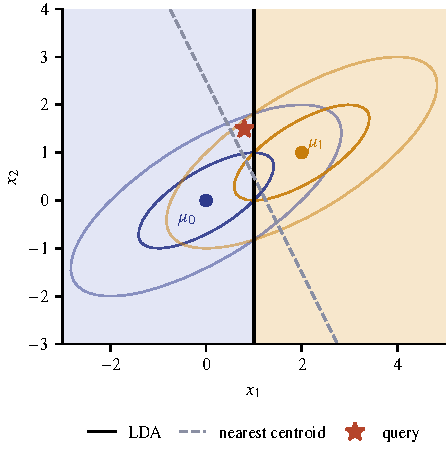
\includegraphics[width=\linewidth]{figures/n6_lda_example.pdf}
\end{minipage}\hfill
\begin{minipage}[c]{0.54\linewidth}
\caption{The LDA worked example. Ellipses are contours of constant Mahalanobis distance ($\Delta = 1, 2$) of the shared
covariance around each mean. The LDA boundary $x_1 = 1$ follows the shape of the classes; the nearest-centroid boundary
(the perpendicular bisector of the means, dashed) ignores it. The query point (star) lies on different sides of the
two boundaries.}
\label{fig:ldaex}
\end{minipage}
\end{figure}


\subsection{Fitting and cost}

Algorithm~\ref{alg:gauss} gives both variants. Following Note~2, Section~6, log-densities are computed with a Cholesky
factor and triangular solves; no matrix is inverted explicitly. A small $\epsilon I$ is added to each covariance
estimate (shrinkage, Note~2, Section~6) so that the factorisation exists even when $n_c \le d$.

\begin{algorithm}[H]
\caption{Gaussian Bayes classifier: QDA (one covariance per class) and LDA (shared covariance)}\label{alg:gauss}
\footnotesize
\begin{algorithmic}[1]
\Require $\{(\x_i, y_i)\}_{i=1}^n$, $\x_i \in \R^d$, $y_i \in \{1, \dots, m\}$; shrinkage $\epsilon \ge 0$; variant $\in$ \{QDA, LDA\}
\Function{Fit}{$\Dtrain$}
  \For{$c = 1, \dots, m$}
    \State $n_c \gets |\{i : y_i = c\}|$, \quad $\hat P_c \gets n_c/n$, \quad $\hat{\vmu}_c \gets \frac{1}{n_c}\sum_{i:\, y_i = c} \x_i$
    \State $\hat\Sigma_c \gets \frac{1}{n_c}\sum_{i:\, y_i = c} (\x_i - \hat{\vmu}_c)(\x_i - \hat{\vmu}_c)\T$ \Comment{$O(n_c d^2)$}
  \EndFor
  \If{variant = QDA}
    \For{$c = 1, \dots, m$}
      \State $L_c \gets \Call{Cholesky}{\hat\Sigma_c + \epsilon I}$, \quad $h_c \gets \sum_{j} \log (L_c)_{jj}$ \Comment{$h_c = \frac12 \log\lvert\Sigma_c\rvert$}
    \EndFor
  \Else \Comment{LDA}
    \State $L \gets \Call{Cholesky}{\sum_c \frac{n_c}{n} \hat\Sigma_c + \epsilon I}$ \Comment{pooled covariance}
    \For{$c = 1, \dots, m$}
      \State $\w_c \gets$ solve $L L\T \w_c = \hat{\vmu}_c$; \quad $b_c \gets -\tfrac12\, \hat{\vmu}_c\T \w_c + \log \hat P_c$ \Comment{\eqref{eq:ldamulti}}
    \EndFor
  \EndIf
\EndFunction
\Function{Predict}{$\x$}
  \For{$c = 1, \dots, m$}
    \If{variant = QDA}
      \State solve $L_c \vect{u} = \x - \hat{\vmu}_c$; \quad $s_c \gets -\tfrac12 \norm{\vect{u}}^2 - h_c + \log \hat P_c$ \Comment{$O(d^2)$}
    \Else
      \State $s_c \gets \w_c\T \x + b_c$ \Comment{$O(d)$}
    \EndIf
  \EndFor
  \State \Return $\argmax_c s_c$ and the softmax of $(s_1, \dots, s_m)$ via log-sum-exp
\EndFunction
\end{algorithmic}
\end{algorithm}

\begin{runtime}{QDA and LDA}
\emph{Training}: class means $O(nd)$; covariances $O(nd^2)$, since every example contributes one $d \times d$ outer
product; Cholesky factorisations $O(d^3)$ each, so $O(md^3)$ for QDA and $O(d^3)$ for LDA, plus $O(md^2)$ for the LDA
solves. Total $O(nd^2 + md^3)$ (QDA) and $O(nd^2 + d^3 + md^2)$ (LDA). \emph{Prediction per query}: QDA needs one
triangular solve per class, $O(md^2)$; LDA only $m$ dot products, $O(md)$. \emph{Memory}: QDA keeps $m$ triangular
factors, $O(md^2)$; trained LDA keeps only $\w_c, b_c$, $O(md)$. \emph{Typical sizes}: for $d = 10^3$ a Cholesky
factorisation takes about $d^3/3 \approx 3 \times 10^8$ operations, a fraction of a second; for $d = 10^4$ each
covariance matrix has $10^8$ entries (0.8~GB in double precision), and QDA with $m = 10$ would need 8~GB, which is why
high-dimensional problems use LDA, diagonal or low-rank covariances. Predictions for a batch of $q$ queries are
matrix--matrix products ($O(qmd)$ for LDA) that run efficiently with BLAS or on a GPU.
\end{runtime}

\paragraph{Counting parameters} QDA in $d$ dimensions estimates $m$ covariance matrices of $d(d+1)/2$ entries each;
LDA one; a diagonal model $md$ variances. For $d = 100$ and $m = 10$ these are about 50\,000, 5\,000 and 1\,000
numbers. More flexible is not automatically better: with few examples per class the shared, shrunk covariance of LDA
often generalises best, an instance of the capacity trade-off of Note~4, Section~5.

\section{Naive Bayes}\label{sec:naive}

\paragraph{From the chain rule to the naive assumption} By the product rule applied repeatedly (the chain rule), the
class density of the $d$ features can always be written as
\[
  p(\x \mid c) = p(x_1 \mid c)\, p(x_2 \mid x_1, c)\, p(x_3 \mid x_1, x_2, c) \cdots p(x_d \mid x_1, \dots, x_{d-1}, c) ,
\]
which is exact but no easier to estimate than $p(\x \mid c)$ itself: the last factor still depends on all $d$
features. Naive Bayes replaces every factor $p(x_j \mid x_1, \dots, x_{j-1}, c)$ by $p(x_j \mid c)$. This is the
assumption of \emph{conditional independence given the class}: for every pair of features,
$p(x_j, x_k \mid c) = p(x_j \mid c)\, p(x_k \mid c)$. It is not the same as ordinary independence (Note~2,
Section~1.1), $p(x_j, x_k) = p(x_j)\, p(x_k)$. Features that are independent within each class are usually dependent overall, through the class: in the
electron/pion table, $P(\text{C = yes}) = 58/200 = 0.29$ and $P(E/p = \text{high}) = 64/200 = 0.32$, whose product
$0.093$ is far from the joint $P(\text{yes, high}) = 36/200 = 0.18$, while within the electrons
$P(\text{yes, high} \mid e) = 0.70$ is close to $P(\text{yes} \mid e)\, P(\text{high} \mid e) = 0.85 \times 0.80 = 0.68$.

The \emph{naive Bayes} classifier therefore uses
\begin{equation}\label{eq:naive}
  p(\x \mid c) = \prod_{j=1}^d p_j(x_j \mid c), \qquad
  s_c(\x) = \log \hat P_c + \sum_{j=1}^d \log \hat p_j(x_j \mid c) ,
\end{equation}
where $p_j(\cdot \mid c)$ is the one-dimensional distribution of feature $j$ in class $c$ and $\hat p_j$ its estimate.
Instead of one density in $d$ dimensions it needs $d$ densities on a line. Each of them is fitted from all $n_c$
examples of the class, so the data do not thin out as $d$ grows (compare Note~3, Section~3), and any one-dimensional
estimator --- a count, a histogram, a kernel estimate (Section~\ref{sec:histnb}) --- can serve. The saving is dramatic:
for $d$ binary features a full table of $p(\x \mid c)$ has $2^d - 1$ free entries per class, about $1.07 \times 10^9$
for $d = 30$, whereas naive Bayes needs only $d = 30$ (for Gaussians, compare the counts at the end of
Section~\ref{sec:gaussian}). Training takes one or two passes over the data (counting, or means and then variances), and
features of different types (binary, counts, categories, real values) can be mixed freely, each with its own
one-dimensional model. In odds form, \eqref{eq:naive} and \eqref{eq:odds} give
\[
  \frac{P(Y = 1 \mid \x)}{P(Y = 0 \mid \x)} = \frac{P_1}{P_0} \prod_{j=1}^d \frac{p_j(x_j \mid 1)}{p_j(x_j \mid 0)} :
\]
each feature contributes its own likelihood ratio, as the two trigger stages did in Section~\ref{sec:odds}. The
subsections below treat binary, count and real-valued features, first with parametric and then with histogram
estimates.

\subsection{Binary features: Bernoulli naive Bayes}\label{sec:bernoulli}

Let $x_j \in \{0, 1\}$ and $\theta_{c,j} = P(x_j = 1 \mid Y = c)$. A compact way to write the Bernoulli probability is
$p_j(x_j \mid c) = \theta_{c,j}^{x_j} (1 - \theta_{c,j})^{1 - x_j}$, which equals $\theta_{c,j}$ for $x_j = 1$ and
$1 - \theta_{c,j}$ for $x_j = 0$.

\paragraph{Maximum likelihood} Let $N_{c,j}$ be the number of class-$c$ examples with $x_j = 1$. The log-likelihood
of $\theta = \theta_{c,j}$ is $N_{c,j} \log\theta + (n_c - N_{c,j}) \log(1 - \theta)$ (the two-category case of Note~2, Section~2.1); its derivative
\[
  \frac{N_{c,j}}{\theta} - \frac{n_c - N_{c,j}}{1 - \theta} = 0
  \quad\Rightarrow\quad \hat\theta_{c,j} = \frac{N_{c,j}}{n_c} ,
\]
the fraction of class-$c$ examples in which the feature is on.

\paragraph{The zero-count problem and Laplace smoothing} If a feature is never on in class $c$ in the training set,
$\hat\theta_{c,j} = 0$, and any future input with $x_j = 1$ gets $p(\x \mid c) = 0$: one feature vetoes the class,
whatever the others say. This is the zero-count problem of maximum-likelihood estimates of categorical
distributions (Note~2, Section~2.1, where pseudo-counts were introduced), and it is common, because with $d$ features and few examples some counts are
always zero. \emph{Laplace smoothing} pretends that each class has been seen $\alpha$ extra times with the feature on
and $\alpha$ extra times with it off:
\begin{equation}\label{eq:laplace}
  \hat\theta_{c,j} = \frac{N_{c,j} + \alpha}{n_c + 2\alpha} , \qquad \alpha > 0 \text{ (usually } \alpha = 1\text{)}.
\end{equation}
The estimate is never $0$ or $1$; it approaches the maximum-likelihood value when $n_c \gg \alpha$ and is pulled towards
$\tfrac12$ when data are scarce. $\alpha$ is a hyperparameter, chosen by validation like any other (Note~4,
Section~7). (An aside for readers who have met Bayesian estimation, Note~8, Section~6: \eqref{eq:laplace} is the
maximum a posteriori estimate under a $\mathrm{Beta}(\alpha + 1, \alpha + 1)$ prior density on $\theta$, a density on
$[0, 1]$ proportional to $\theta^{\alpha}(1 - \theta)^{\alpha}$.)

\begin{worked}{Bernoulli naive Bayes for jet tagging, with and without smoothing}
Jets are labelled $b$ (from a bottom quark, $y = 1$) or light ($y = 0$, subscript $\mathrm{lt}$) using three binary features: a displaced
secondary vertex was found ($x_1$), a soft lepton was found inside the jet ($x_2$), the track multiplicity is high
($x_3$). Eight training jets:

\begin{center}\small
\begin{tabular}{@{}lcccc@{\qquad}lcccc@{}}\toprule
jet & $x_1$ & $x_2$ & $x_3$ & $y$ & jet & $x_1$ & $x_2$ & $x_3$ & $y$ \\ \midrule
1 & 1 & 1 & 1 & $b$ & 5 & 0 & 0 & 0 & light \\
2 & 1 & 0 & 1 & $b$ & 6 & 1 & 0 & 0 & light \\
3 & 1 & 0 & 0 & $b$ & 7 & 0 & 1 & 0 & light \\
4 & 0 & 0 & 1 & light & 8 & 0 & 0 & 1 & light \\ \bottomrule
\end{tabular}
\end{center}

\emph{Priors}: $\hat P_b = 3/8$, $\hat P_{\mathrm{lt}} = 5/8$.
\emph{Counts}: in the 3 $b$-jets, $N = (3, 1, 2)$; in the 5 light jets, $N = (1, 1, 2)$.

\emph{Without smoothing} ($\alpha = 0$): $\hat\theta_b = (1, \tfrac13, \tfrac23)$, $\hat\theta_{\mathrm{lt}} = (\tfrac15, \tfrac15, \tfrac25)$.
\begin{itemize}
\item Query $\x = (1, 1, 0)$: $\hat p(\x \mid b) = 1 \cdot \tfrac13 \cdot \tfrac13 = \tfrac19$ and
$\hat p(\x \mid \mathrm{lt}) = \tfrac15 \cdot \tfrac15 \cdot \tfrac35 = \tfrac{3}{125}$. Times the priors: $\tfrac19 \cdot \tfrac38 = 0.0417$ and
$\tfrac{3}{125} \cdot \tfrac58 = 0.0150$, so $\hat P(b \mid \x) = 0.0417/0.0567 = 25/34 = 0.74$.
\item Query $\x = (0, 1, 1)$: $\hat p(\x \mid b) = (1 - 1) \cdot \tfrac13 \cdot \tfrac23 = 0$, so $\hat P(b \mid \x) = 0$
exactly. Every training $b$-jet had a vertex, so a $b$-jet without one is declared impossible --- a certainty
based on three examples.
\end{itemize}

\emph{With Laplace smoothing} ($\alpha = 1$): $\hat\theta_b = (\tfrac{3+1}{3+2}, \tfrac{1+1}{5}, \tfrac{2+1}{5}) = (0.8, 0.4, 0.6)$
and $\hat\theta_{\mathrm{lt}} = (\tfrac27, \tfrac27, \tfrac37)$.
\begin{itemize}
\item $\x = (1, 1, 0)$: $\hat p(\x \mid b) = 0.8 \cdot 0.4 \cdot 0.4 = 0.128$, $\hat p(\x \mid \mathrm{lt}) = \tfrac27 \cdot \tfrac27 \cdot \tfrac47 = 0.0466$;
times priors $0.0480$ and $0.0292$; $\hat P(b \mid \x) = 0.62$.
\item $\x = (0, 1, 1)$: $\hat p(\x \mid b) = 0.2 \cdot 0.4 \cdot 0.6 = 0.048$, $\hat p(\x \mid \mathrm{lt}) = \tfrac57 \cdot \tfrac27 \cdot \tfrac37 = 0.0875$;
times priors $0.0180$ and $0.0547$; $\hat P(b \mid \x) = 0.25$.
\end{itemize}
Smoothing removes the veto (the second jet is now merely unlikely to be a $b$-jet) and makes the first posterior less
extreme ($0.74 \to 0.62$): with three $b$-jets, the data do not justify strong conclusions.
\end{worked}

\paragraph{Naive Bayes is linear in the log-odds} Take the logarithm of the Bernoulli probability:
\[
  \log p_j(x_j \mid c) = x_j \log\theta_{c,j} + (1 - x_j)\log(1 - \theta_{c,j})
  = x_j \log\frac{\theta_{c,j}}{1 - \theta_{c,j}} + \log(1 - \theta_{c,j}) .
\]
Sum over $j$, add $\log P_c$, and subtract the scores of the two classes:
\begin{equation}\label{eq:nblinear}
  \log\frac{P(Y = 1 \mid \x)}{P(Y = 0 \mid \x)} = \w\T\x + b, \qquad
  w_j = \log\frac{\theta_{1,j}(1 - \theta_{0,j})}{\theta_{0,j}(1 - \theta_{1,j})}, \qquad
  b = \log\frac{P_1}{P_0} + \sum_{j=1}^d \log\frac{1 - \theta_{1,j}}{1 - \theta_{0,j}} .
\end{equation}
Bernoulli naive Bayes is therefore a linear classifier, with posterior $\sigma(\w\T\x + b)$. Each weight is a log
odds ratio: how much more often the feature is on in class~1 than in class~0, on the odds scale. In the smoothed jet
example, $w_1 = \log\frac{0.8 \cdot 5/7}{2/7 \cdot 0.2} = \log 10 = 2.30$, $w_2 = \log\tfrac53 = 0.51$,
$w_3 = \log 2 = 0.69$ and $b = \log\tfrac35 + \log\tfrac{7}{25} + \log\tfrac{21}{25} + \log\tfrac{7}{10} = -2.31$. For
$\x = (1, 1, 0)$: $2.30 + 0.51 - 2.31 = 0.50$ and $\sigma(0.50) = 0.62$, as before. The vertex feature dominates, as
the physics suggests.

\begin{algorithm}[H]
\caption{Bernoulli naive Bayes with Laplace smoothing}\label{alg:bnb}
\footnotesize
\begin{algorithmic}[1]
\Require binary data $\x_i \in \{0, 1\}^d$, labels $y_i \in \{1, \dots, m\}$, smoothing $\alpha > 0$
\Function{Fit}{$\Dtrain$, $\alpha$}
  \For{$c = 1, \dots, m$}
    \State $n_c \gets |\{i : y_i = c\}|$, \quad $\hat P_c \gets n_c / n$
    \State $N_{c,j} \gets \sum_{i:\, y_i = c} x_{ij}$ for $j = 1, \dots, d$ \Comment{one pass over the data}
    \State $\theta_{c,j} \gets (N_{c,j} + \alpha)/(n_c + 2\alpha)$ \Comment{\eqref{eq:laplace}}
    \State $\omega_{c,j} \gets \log\big(\theta_{c,j}/(1 - \theta_{c,j})\big)$; \quad $\beta_c \gets \log \hat P_c + \sum_j \log(1 - \theta_{c,j})$
  \EndFor
\EndFunction
\Function{Predict}{$\x$}
  \State $s_c \gets \beta_c + \sum_{j:\, x_j = 1} \omega_{c,j}$ for $c = 1, \dots, m$ \Comment{only the features that are on}
  \State \Return $\argmax_c s_c$ and the softmax of $(s_1, \dots, s_m)$ via log-sum-exp
\EndFunction
\end{algorithmic}
\end{algorithm}

\begin{runtime}{Bernoulli naive Bayes}
\emph{Training}: $O(nd)$, a single pass that adds each example to the counts of its own class, plus $O(md)$ to turn
counts into logarithms. No iterations, no optimisation. \emph{Prediction per query}: $O(md)$ for a dense input; with the
precomputed $\beta_c$ only the features that are on are visited, $O(mk)$ for $k$ non-zero features --- the reason
naive Bayes is fast on sparse text data. \emph{Memory}: $O(md)$. A batch of queries is one matrix product
$X \Omega\T$ (with $\Omega$ the $m \times d$ table of the $\omega_{c,j}$) plus a bias, $O(qmd)$.
\end{runtime}

\subsection{Counts: multinomial naive Bayes}\label{sec:multinomial}

For a document represented by word counts (the bag of words of Note~1, Section~3), the \emph{multinomial} model treats
each of its $L$ tokens as an independent draw from a class-specific distribution $\pi_{c,1}, \dots, \pi_{c,V}$ over a
vocabulary of $V$ words. If word $v$ occurs $a_v$ times in the document, the order of the words does not matter and
\[
  s_c = \log P_c + \sum_{v=1}^V a_v \log \pi_{c,v} + \text{const},
\]
where the constant $\log\big(L!/\prod_v a_v!\big)$ counts the orderings of the words; it does not depend on $c$ and
cancels in every comparison. The score is again linear, now in the counts. The maximum-likelihood estimate, derived with a Lagrange multiplier exactly like
the priors in Section~\ref{sec:bayes}, is $\hat\pi_{c,v} = N_{c,v} / N_c$, where $N_{c,v}$ is the number of times word
$v$ occurs in the training documents of class $c$ and $N_c = \sum_v N_{c,v}$ their total length. A word never seen in a
class would get $\hat\pi_{c,v} = 0$ and veto the class; Laplace smoothing adds $\alpha$ to every count,
\begin{equation}\label{eq:multsmooth}
  \hat\pi_{c,v} = \frac{N_{c,v} + \alpha}{N_c + \alpha V} .
\end{equation}
The Bernoulli model records only whether a word occurs; the multinomial model also uses how often. On text
classification benchmarks the multinomial model usually works better, especially with large
vocabularies~\cite{mccallum1998}.

\needspace{14\baselineskip}
\begin{worked}{multinomial naive Bayes on short abstracts}
Classify very short abstracts as particle physics (hep) or astrophysics (astro) with the vocabulary
\{quark, jet, collider, galaxy, star, redshift\}, $V = 6$, and six training documents,

hep: ``quark jet jet'', ``collider quark'', ``jet collider''; astro: ``galaxy star'', ``star redshift galaxy'',
``jet galaxy''. Counting the tokens of each class gives the table of word counts $N_{c,v}$:

\begin{center}\small
\begin{tabular}{@{}lccccccc@{}}\toprule
class & quark & jet & collider & galaxy & star & redshift & total $N_c$ \\ \midrule
hep & 2 & 3 & 2 & 0 & 0 & 0 & 7 \\
astro & 0 & 1 & 0 & 3 & 2 & 1 & 7 \\ \bottomrule
\end{tabular}
\end{center}

Priors are $\tfrac12$ each. With $\alpha = 1$, \eqref{eq:multsmooth} divides by $7 + 6 = 13$:
\[
  \hat\pi_{\mathrm{hep}} = \tfrac{1}{13}(3, 4, 3, 1, 1, 1), \qquad
  \hat\pi_{\mathrm{astro}} = \tfrac{1}{13}(1, 2, 1, 4, 3, 2) .
\]
Each token contributes its log ratio $\log(\hat\pi_{\mathrm{hep},v}/\hat\pi_{\mathrm{astro},v})$:
quark $\log 3$, jet $\log 2$, galaxy $\log\tfrac14$, star $\log\tfrac13$.
\begin{itemize}
\item ``jet jet star'': log-odds $= 2\log 2 - \log 3 = 0.29$, i.e.\ odds $\tfrac42 \cdot \tfrac42 \cdot \tfrac13 = \tfrac43$, so
$P(\mathrm{hep}) = (4/3)/(1 + 4/3) = \tfrac47 = 0.57$.
Without smoothing, $\hat\pi_{\mathrm{hep,star}} = 0$ and the answer would be astro with certainty, although two of the
three words point to hep.
\item ``quark star jet'': log-odds $= \log 3 - \log 3 + \log 2 = \log 2$, so $P(\mathrm{hep}) = \tfrac23$. Without
smoothing \emph{both} likelihoods are zero (quark never occurs in astro, star never in hep) and the posterior is
$0/0$, undefined.
\item ``jet galaxy'': log-odds $= \log 2 - \log 4 = -\log 2$, so $P(\mathrm{hep}) = \tfrac13$: astro.
\end{itemize}
Words outside the vocabulary are simply skipped. Note that ``jet'' is evidence for hep but not proof: astrophysical
jets exist, and the smoothed model keeps that possibility open.
\end{worked}

\begin{algorithm}[H]
\caption{Multinomial naive Bayes for documents (bag of words)}\label{alg:mnb}
\footnotesize
\begin{algorithmic}[1]
\Require documents as token lists over a vocabulary of size $V$, labels $y_i \in \{1, \dots, m\}$, smoothing $\alpha > 0$
\Function{Fit}{documents, labels, $\alpha$}
  \State $N_{c,v} \gets 0$ for all $c, v$; \quad $n \gets$ number of documents
  \For{each document $i$ and each token $v$ in it}
    \State $N_{y_i, v} \gets N_{y_i, v} + 1$ \Comment{one pass over all $T$ tokens}
  \EndFor
  \For{$c = 1, \dots, m$}
    \State $n_c \gets$ number of documents with $y_i = c$; \quad $\hat P_c \gets n_c/n$; \quad $N_c \gets \sum_v N_{c,v}$
    \State $q_{c,v} \gets \log(N_{c,v} + \alpha) - \log(N_c + \alpha V)$ for all $v$ \Comment{log of \eqref{eq:multsmooth}}
  \EndFor
\EndFunction
\Function{Predict}{document $t_1, \dots, t_L$}
  \State $s_c \gets \log \hat P_c + \sum_{k=1}^{L} q_{c, t_k}$ for $c = 1, \dots, m$ \Comment{skip tokens outside the vocabulary}
  \State \Return $\argmax_c s_c$ and the softmax of $(s_1, \dots, s_m)$ via log-sum-exp
\EndFunction
\end{algorithmic}
\end{algorithm}

\begin{runtime}{multinomial naive Bayes}
With $T$ tokens in the training set and $L$ tokens in a query document: \emph{training} $O(T + mV)$, one pass to count
plus one logarithm per table entry; \emph{prediction} $O(mL)$, one table look-up per token and class;
\emph{memory} $O(mV)$, e.g.\ $4 \times 10^4$ numbers for $m = 2$ and $V = 20\,000$. Nothing depends on $V$ at prediction
time; cheap training and prediction made it practical for filtering mail on modest hardware. A batch of $q$ documents
is one sparse $q \times V$ count matrix times the $V \times m$ table of logarithms.
\end{runtime}

\subsection{Real-valued features: Gaussian naive Bayes}\label{sec:gnb}

For continuous features the simplest choice is a one-dimensional Gaussian per class and feature,
$p_j(x_j \mid c) = \Normal(x_j; \mu_{c,j}, \sigma_{c,j}^2)$, fitted by the class means and variances of each column. This is
QDA with \emph{diagonal} covariance matrices: $d$ variances per class instead of $d(d+1)/2$ covariances. The log-score
\[
  s_c(\x) = \log P_c - \sum_{j=1}^d \left[\frac{(x_j - \mu_{c,j})^2}{2\sigma_{c,j}^2} + \tfrac12 \log \sigma_{c,j}^2\right]
  + \text{const}
\]
is quadratic in $\x$ but has no cross terms $x_j x_k$: the boundary is a quadric whose axes are aligned with the
coordinate axes. If the variances do not depend on the class ($\sigma_{c,j} = \sigma_j$), the $x_j^2$ terms cancel and
the classifier is linear, as in LDA.

\begin{worked}{Gaussian naive Bayes on a small table}
Two kinds of events, A and B, are described by two measured quantities $(x_1, x_2)$; four events of each kind, equal
priors:

\begin{center}\small
\begin{tabular}{@{}lcccc@{\qquad}cc@{}}\toprule
class & \multicolumn{4}{c}{training points $(x_1, x_2)$} & means & variances \\ \midrule
A & $(1, 2)$ & $(3, 4)$ & $(3, 2)$ & $(5, 4)$ & $(3, 3)$ & $(2, 1)$ \\
B & $(5, 6)$ & $(7, 4)$ & $(7, 8)$ & $(9, 6)$ & $(7, 6)$ & $(2, 2)$ \\ \bottomrule
\end{tabular}
\end{center}

For example, the $x_1$ values of A are $1, 3, 3, 5$: mean $3$, variance $\tfrac14(4 + 0 + 0 + 4) = 2$ (dividing by
$n_c$, the maximum-likelihood estimate). Dropping the common terms $\log P_c$ and $\log 2\pi$, each class scores
$-\big[\text{sum of } (x_j - \mu_{c,j})^2/(2\sigma_{c,j}^2)\big] - \tfrac12 \sum_j \log \sigma_{c,j}^2$.
\begin{itemize}
\item Query $(5, 5)$. A: $\tfrac{(5-3)^2}{4} + \tfrac{(5-3)^2}{2} = 1 + 2 = 3$, and $\tfrac12(\log 2 + \log 1) = 0.347$, so
$s_A = -3.347$. B: $\tfrac{(5-7)^2}{4} + \tfrac{(5-6)^2}{4} = 1 + 0.25 = 1.25$, and $\tfrac12(\log 2 + \log 2) = 0.693$,
so $s_B = -1.943$. Log-odds $s_B - s_A = 1.40$ and $P(B \mid \x) = \sigma(1.40) = 0.80$: class B.
\item Query $(6, 3)$. A: $\tfrac{9}{4} + 0 = 2.25$, $s_A = -2.597$. B: $\tfrac14 + \tfrac94 = 2.5$, $s_B = -3.193$.
Log-odds $-0.60$, $P(B \mid \x) = 0.36$: class A. The point is nearer B in $x_1$, but its $x_2$ sits exactly on A's mean
and B is broad in $x_2$, so the second feature decides.
\end{itemize}
\end{worked}

\begin{algorithm}[H]
\caption{Gaussian naive Bayes}\label{alg:gnb}
\footnotesize
\begin{algorithmic}[1]
\Require real data $\x_i \in \R^d$, labels $y_i \in \{1, \dots, m\}$, variance floor $\epsilon > 0$
\Function{Fit}{$\Dtrain$}
  \For{$c = 1, \dots, m$}
    \State $n_c \gets |\{i : y_i = c\}|$, \quad $\hat P_c \gets n_c/n$
    \For{$j = 1, \dots, d$}
      \State $\mu_{c,j} \gets \frac{1}{n_c}\sum_{i:\, y_i = c} x_{ij}$, \quad $\sigma^2_{c,j} \gets \frac{1}{n_c}\sum_{i:\, y_i = c} (x_{ij} - \mu_{c,j})^2 + \epsilon$
    \EndFor
  \EndFor
\EndFunction
\Function{Predict}{$\x$}
  \State $s_c \gets \log \hat P_c - \sum_{j} \big[(x_j - \mu_{c,j})^2/(2\sigma^2_{c,j}) + \tfrac12 \log(2\pi\sigma^2_{c,j})\big]$ for $c = 1, \dots, m$
  \State \Return $\argmax_c s_c$ and the softmax of $(s_1, \dots, s_m)$ via log-sum-exp
\EndFunction
\end{algorithmic}
\end{algorithm}

\begin{runtime}{Gaussian naive Bayes}
\emph{Training}: $O(nd)$, one pass for the means and one for the variances (or a single pass with a running-variance
update). \emph{Prediction per query}: $O(md)$; a batch of $q$ queries costs $O(qmd)$ in a few broadcast array
operations (of order a second in numpy for $q = 10^5$, $m = 10$, $d = 100$). \emph{Memory}: $O(md)$ for the means and variances. Compared with QDA,
the factor $d^2$ in training and prediction and the $d^3$ factorisation disappear; the floor $\epsilon$ (often a tiny
fraction of the largest feature variance) prevents division by zero when a feature is constant within a class.
\end{runtime}

\subsection{Real-valued features without a shape assumption: histogram naive Bayes}\label{sec:histnb}

A Gaussian per feature is itself an assumption, and skewed, bounded or two-peaked features fit it badly. Because
every density in \eqref{eq:naive} is one-dimensional, a non-parametric estimate is affordable: the curse of
dimensionality of Note~3, Section~3, never arises. The simplest is a histogram (Note~3, Section~1). For each feature
$j$ fix $K$ bins of width $h_j$ (Note~3 calls the number of bins $m$; here $m$ counts classes), the \emph{same} bins for every class, and let $N_{c,j,b}$ be the number of class-$c$
examples whose $x_j$ falls in bin $b$. With Laplace smoothing, for $x_j$ in bin $b$,
\begin{equation}\label{eq:histnb}
  \hat p_j(x_j \mid c) = \frac{N_{c,j,b} + \alpha}{n_c + \alpha K} \cdot \frac{1}{h_j} .
\end{equation}
The first factor is the smoothed probability of the bin, the second turns it into a density. Since the bins are shared,
$1/h_j$ is common to all classes and cancels in every comparison. The number of bins is chosen as in Note~3, Section~1,
or by validation. Replacing each histogram by a one-dimensional kernel density estimate (Note~5, Section~4) gives
\emph{kernel naive Bayes}: smoother estimates, at the price of keeping the training data.

\begin{worked}{histogram naive Bayes on the same table}
Take the A/B table of the Gaussian example and three bins per feature: for $x_1$ the bins $[0, 4)$, $[4, 8)$, $[8, 12)$
($h_1 = 4$), for $x_2$ the bins $[1, 4)$, $[4, 7)$, $[7, 10)$ ($h_2 = 3$). The bin counts are
\begin{center}\small
\begin{tabular}{@{}lcc@{}}\toprule
class & $x_1$: counts in bins 1, 2, 3 & $x_2$: counts in bins 1, 2, 3 \\ \midrule
A & $3, 1, 0$ & $2, 2, 0$ \\
B & $0, 3, 1$ & $0, 3, 1$ \\ \bottomrule
\end{tabular}
\end{center}
With $\alpha = 1$ and $K = 3$ every class divides by $n_c + \alpha K = 4 + 3 = 7$; the widths cancel and are dropped.
\begin{itemize}
\item Query $(5, 5)$, bins $(2, 2)$. A: $\tfrac{1+1}{7} \cdot \tfrac{2+1}{7} = \tfrac{6}{49}$; B:
$\tfrac{3+1}{7} \cdot \tfrac{3+1}{7} = \tfrac{16}{49}$. Equal priors, so $P(B \mid \x) = 16/22 = 0.73$: class B
(Gaussian naive Bayes: $0.80$).
\item Query $(6, 3)$, bins $(2, 1)$. A: $\tfrac27 \cdot \tfrac37 = \tfrac{6}{49}$; B: $\tfrac47 \cdot \tfrac17 =
\tfrac{4}{49}$, so $P(B \mid \x) = 4/10 = 0.40$: class A (Gaussian naive Bayes: $0.36$).
\end{itemize}
Both decisions agree with the Gaussian model, without assuming any shape. Without smoothing the second query would
get $P(B \mid \x) = 0$, because no B example has $x_2$ in bin~1: the zero-count veto of Section~\ref{sec:bernoulli}
again, now for a continuous feature.
\end{worked}

\begin{algorithm}[H]
\caption{Histogram naive Bayes}\label{alg:hnb}
\footnotesize
\begin{algorithmic}[1]
\Require real data $\x_i \in \R^d$, labels $y_i \in \{1, \dots, m\}$; for each feature a start $a_j$ and width $h_j$ of $K$ bins; $\alpha > 0$
\Function{Bin}{$x_j$}
  \State \Return $\min\big(K, \max(1, \lfloor (x_j - a_j)/h_j \rfloor + 1)\big)$ \Comment{values outside go to the end bins}
\EndFunction
\Function{Fit}{$\Dtrain$, $\alpha$}
  \State $N_{c,j,b} \gets 0$ for all $c, j, b$
  \For{$i = 1, \dots, n$ and $j = 1, \dots, d$}
    \State $b \gets \Call{Bin}{x_{ij}}$; \quad $N_{y_i, j, b} \gets N_{y_i, j, b} + 1$ \Comment{one pass over the data}
  \EndFor
  \For{$c = 1, \dots, m$}
    \State $n_c \gets |\{i : y_i = c\}|$, \quad $\hat P_c \gets n_c/n$
    \State $q_{c,j,b} \gets \log(N_{c,j,b} + \alpha) - \log(n_c + \alpha K) - \log h_j$ for all $j, b$ \Comment{log of \eqref{eq:histnb}}
  \EndFor
\EndFunction
\Function{Predict}{$\x$}
  \State $b_j \gets \Call{Bin}{x_j}$ for $j = 1, \dots, d$ \Comment{shared by all classes}
  \State $s_c \gets \log \hat P_c + \sum_{j} q_{c,j,b_j}$ for $c = 1, \dots, m$
  \State \Return $\argmax_c s_c$ and the softmax of $(s_1, \dots, s_m)$ via log-sum-exp
\EndFunction
\end{algorithmic}
\end{algorithm}

\begin{runtime}{histogram and kernel naive Bayes}
\emph{Training}: $O(nd)$ to bin and count every entry once, plus $O(mdK)$ to turn the counts into logarithms.
\emph{Prediction per query}: $O(d)$ to find the bins (one division each for equal widths; $O(d \log K)$ by binary
search when the bin edges are arbitrary), plus $O(md)$ table look-ups, so $O(md)$ in total. \emph{Memory}: $O(mdK)$,
the count tables. Kernel naive Bayes only stores the data, $O(nd)$ time and memory, but evaluates, for each
class and feature, a one-dimensional sum over the $n_c$ training values: $O(nd)$ per query, like the
multidimensional kernel classifier, though without its curse of dimensionality.
\end{runtime}

\subsection{The price of independence}

Naive Bayes buys speed and immunity to the curse of dimensionality with capacity. The model cannot represent any
interaction between features within a class: in the right-hand panel of Figure~\ref{fig:bayesgauss}, where the classes
differ only through the correlation between $x_1$ and $x_2$, naive Bayes has 48.6\% test error, no better than
guessing, while a Gaussian Bayes classifier with full covariances reaches 20.9\% on the same data. Both use the same
Bayes rule; the factorised density simply has no parameter that could register the sign of a correlation. So ``naive
Bayes'' names one cheap, low-capacity choice of class densities, not the Bayes classifier as such, whose capacity is
whatever its density estimator allows. The second price concerns probabilities rather than decisions. The decisions of naive Bayes can be
optimal even when its probability estimates are poor~\cite{domingos1997}; in practice its estimates are pushed towards
$0$ and $1$~\cite{niculescu2005}, because correlated evidence is counted several times. The extreme case is a
duplicated feature. If the vertex feature $x_1$ of the jet example
were entered twice, the likelihood ratio of $\x = (1, 1, 0)$ would gain a second factor
$\theta_{b,1}/\theta_{\mathrm{lt},1} = 0.8/(2/7) = 2.8$ for the copy (which is on). The log-odds would grow by
$\log 2.8 = 1.03$ (in the form \eqref{eq:nblinear}: $w_1$ for the new weight plus $\log\tfrac{7}{25}$ for the new bias
term), from $0.50$ to $1.53$, and the posterior would rise from $0.62$ to $0.82$, although no new information was
added.

\paragraph{Missing features} A practical strength of the factorised model: if feature $j$ is not measured for an input
(a detector channel was off) for reasons unrelated to the class (missing at random), the correct generative treatment
marginalises over it,
$\int p_j(x_j \mid c)\, dx_j = 1$, which simply removes the $j$-th factor from \eqref{eq:naive}. No imputation is
needed.

\begin{modern}{a baseline that refuses to die}
Many statistical spam filters around 2000 were naive Bayes classifiers on word occurrences or
counts~\cite{sahami1998}, and the method remains a strong baseline for text: on sentiment and topic benchmarks, naive Bayes features combined with a linear classifier rivalled far more
complex models of the time~\cite{wang2012}. A common first attempt today on a small labelled text dataset is a linear
classifier on embeddings from a pre-trained model (Note~9); comparing against naive Bayes on raw counts shows how much
the representation actually adds.
\end{modern}

\section{Generative and discriminative classifiers}\label{sec:gendisc}

The Bayes classifier is \emph{generative}: it models how the inputs of each class are generated, i.e.\ the joint
distribution $p(\x, c) = p(\x \mid c)\,P(Y = c)$, and derives $P(Y \mid \x)$ from it. Given $p(\x, c)$ for every $c$, the
posterior $P(Y = c \mid \x) = p(\x, c) / \sum_{c'} p(\x, c')$ is the slice at $\x$ rescaled to sum to one: the class
probabilities are proportional to the joint probabilities, and the denominator is only a normaliser --- in the electron/pion example, a row of counts over its total. A
\emph{discriminative} classifier, such as logistic regression (Note~9), models $P(Y \mid \x)$ directly and never
describes the inputs. The trade-off is classical. Generative models make stronger assumptions, need fewer examples
to reach their best performance, handle missing features by marginalisation, and can in principle flag inputs with
low $p(\x)$ as unusual (for high-dimensional deep generative models low likelihood is an unreliable outlier
signal~\cite{nalisnick2019}); discriminative models spend all their capacity on the decision and usually win when data are
plentiful. For naive Bayes against logistic regression, the generative model approaches its (higher) asymptotic error
faster, the discriminative one reaches a lower error eventually~\cite{ng2002}.

LDA and logistic regression make the point sharply. Both produce posteriors $\sigma(\w\T\x + b)$
(Section~\ref{sec:gaussian}), and Bernoulli naive Bayes does too \eqref{eq:nblinear}. LDA reads $\w$ off fitted Gaussians
via \eqref{eq:lda} --- in closed form, from $2d + d(d+1)/2 + 1$ estimated numbers --- and is right if the classes really
are Gaussian with a shared covariance. Logistic regression fits the $d + 1$ numbers of $\w$ and $b$ to the labels by
iterative optimisation (gradient descent or Newton's method, Note~7, Sections~3 and~6), and remains sensible whenever the log-odds are linear, whatever the class densities.
Missing features show the difference in practice. A discriminative model is a formula $f(\x)$ that needs every
component of $\x$; if $x_j$ is missing there is no density over $x_j$ to integrate out, so $x_j$ must first be guessed
(\emph{imputed}), for instance by its training mean, whereas naive Bayes simply drops the factor $p_j(x_j \mid c)$
(Section~\ref{sec:naive}). Table~\ref{tab:gendisc} summarises the contrast.

\begin{table}[htbp]\centering\small
\caption{Generative and discriminative classifiers at a glance.}
\label{tab:gendisc}
\renewcommand{\arraystretch}{1.1}
\begin{tabular}{@{}L{0.25\linewidth}L{0.33\linewidth}L{0.33\linewidth}@{}}\toprule
 & generative (Bayes classifier, LDA, naive Bayes) & discriminative (logistic regression, SVM) \\ \midrule
models & $p(\x \mid c)$ and $P(c)$ & $P(c \mid \x)$ or only the boundary \\
training & counting and averaging, closed form & iterative optimisation \\
small $n$ & good, if the assumptions hold & may overfit \\
large $n$ & limited by wrong assumptions & usually better \\
missing features & marginalise & needs imputation \\
unusual inputs & low $p(\x)$ may flag them & no notion of $p(\x)$ \\
new class balance & change $P(c)$ & rescale odds (Section~\ref{sec:odds}) \\ \bottomrule
\end{tabular}
\end{table}

\begin{modern}{generative models as classifiers}
Every model that assigns a likelihood to data can be turned into a classifier by \eqref{eq:bayes}. A text-to-image
diffusion model (Note~2, Section~5) estimates how well an image fits each candidate caption; choosing the caption with
the best fit gives a zero-shot image classifier with competitive accuracy and strong compositional reasoning; a
class-conditional version trained on ImageNet also proved robust to some distribution shifts~\cite{li2023}. A language
model can be used generatively in the same way, by scoring the probability of the input text given each label and
combining it with a prior (``noisy-channel'' scoring). These are Bayes classifiers with a billion parameters or more in
the density estimator.
\end{modern}

\section{Running times at a glance}\label{sec:cost}

Table~\ref{tab:cost} collects the costs of the running-time boxes ($k$ non-zero features, $V$ vocabulary size, $T$
training tokens, $L$ tokens in a query document, $K$ bins per feature): only full covariances cost $d^2$ or $d^3$, and only the
kernel-density versions (full and naive) pay per query for the size of the training set.

\begin{table}[h!]\centering\footnotesize
\caption{Training time, prediction time per query and memory of the classifiers of this note.}
\label{tab:cost}
\renewcommand{\arraystretch}{1.1}
\begin{tabular}{@{}L{0.3\linewidth}L{0.22\linewidth}L{0.2\linewidth}L{0.17\linewidth}@{}}\toprule
classifier & training & prediction & memory \\ \midrule
Bayes with KDE (Note~5, Sec.~4) & $O(nd)$ (store data) & $O(nd)$ & $O(nd)$ \\
QDA & $O(nd^2 + md^3)$ & $O(md^2)$ & $O(md^2)$ \\
LDA & $O(nd^2 + d^3 + md^2)$ & $O(md)$ & $O(md)$ \\
Gaussian naive Bayes & $O(nd)$ & $O(md)$ & $O(md)$ \\
Histogram naive Bayes & $O(nd + mdK)$ & $O(md)$ & $O(mdK)$ \\
Kernel naive Bayes & $O(nd)$ (store data) & $O(nd)$ & $O(nd)$ \\
Bernoulli naive Bayes & $O(nd)$ & $O(md)$, sparse $O(mk)$ & $O(md)$ \\
Multinomial naive Bayes & $O(T + mV)$ & $O(mL)$ & $O(mV)$ \\ \bottomrule
\end{tabular}
\end{table}

\needspace{14\baselineskip}
\begin{keyidea}[Summary]
The Bayes classifier fits a density to each class and a prior, and combines them with Bayes' rule; fitting each class
separately and using class frequencies as priors is maximum likelihood. Compute in log space and normalise with
log-sum-exp. Posterior odds equal the likelihood ratio times the prior odds: rare classes need strong evidence, and
unequal costs move the threshold in the same way as priors. Gaussian class densities give quadratic boundaries (QDA,
possibly two thresholds in one dimension), or linear ones when the covariance is shared (LDA, with logistic
posteriors), which reduces to nearest centroid in the simplest case. Naive Bayes assumes independent features within
each class: one or two passes over the data, one-dimensional estimates, no curse, low capacity and overconfident probabilities;
with binary or count features it is linear in the log-odds, and Laplace smoothing prevents a single zero count from
vetoing a class. Generative classifiers model the inputs; discriminative ones model only the decision.
\end{keyidea}

\begin{questions}
\begin{conceptual}
\item A binary classifier outputs a number $g(\x) \in [0, 1]$ that estimates $P(Y = 1 \mid \x)$. Why is the cut
$g(\x) > \tfrac12$ the natural one, and why is a single score with a cut equivalent to comparing two class scores
$g_1(\x)$ and $g_0(\x)$? When would you choose a cut other than $\tfrac12$?
\item Explain in your own words the roles of the likelihood $p(\x \mid c)$, the prior $P(c)$ and the posterior
$P(c \mid \x)$ in a Bayes classifier. Through which of them does the new input $\x$ enter, and which one do we need in
order to decide?
\item True or false, with a justification: ``If a trigger accepts 95\% of signal events, then an accepted event is a
signal event with probability 0.95.''
\item Why can the denominator of Bayes' rule be ignored when we only want a decision? Give a situation in which it is
needed.
\item A naive Bayes model multiplies 1000 per-feature probabilities. What goes wrong numerically if this is done
literally, and how do log-scores and the log-sum-exp trick fix it?
\item Background and signal are unit-variance Gaussian classes centred at $0$ and $2.5$. The prior of signal is
increased while the class densities stay the same. Does the likelihood ratio change? In which direction does the
decision boundary move, and why?
\item Explain why making a missed signal ten times more costly has the same effect on the decision as making the prior
odds of signal ten times larger. Why is this almost, but not exactly, the same as making signal ten times more common?
\item Why does a Bayes classifier with Gaussian class densities have a quadratic boundary in general, and which
assumption makes it linear? Which term of the log-score cancels?
\item In one dimension, two Gaussian classes have different variances. Explain without calculation why the class with
the smaller variance can lose in both tails, so that its decision region is an interval.
\item Under which assumptions does LDA reduce to the nearest-centroid classifier? Two classes share the covariance
$\Sigma$ with $\Sigma_{11} = 2$, $\Sigma_{12} = \Sigma_{21} = \Sigma_{22} = 1$, have means $(0, 0)$ and $(2, 1)$ and equal
priors; LDA turns out to use only $x_1$. Explain why $x_2$ carries no extra information although its mean differs between
the classes, and why nearest centroid can classify a point such as $(0.8, 1.5)$ differently.
\item ``Bayes classifier'' and ``naive Bayes'' are not synonyms. Explain the difference and say which has the larger
capacity and why.
\item Describe a two-class dataset on which naive Bayes performs no better than guessing although a Bayes classifier
with full covariance matrices works well. What property of the data is invisible to naive Bayes, and why do the
boundaries of Gaussian naive Bayes never contain cross terms $x_j x_k$?
\item Why are the posterior probabilities of naive Bayes often overconfident even when its decisions are good? What
happens to the log-odds if one feature is copied into the input twice?
\item For classifying physics abstracts by their words, what information does the multinomial model use that the
Bernoulli model ignores? Give an example of two documents that the Bernoulli model cannot tell apart.
\item What is the zero-count problem? How does Laplace smoothing solve it, and what happens to the estimates
$\hat\theta_{c,j}$ when $\alpha \to \infty$?
\item How does a generative classifier handle an input with a missing feature? Why is this particularly simple for naive
Bayes, and why is it harder for a discriminative model such as logistic regression?
\item You have 20 labelled examples with 50 features. Would you use naive Bayes or a discriminative linear classifier
such as logistic regression (Note~9)? Would plain LDA, without shrinkage, work here (how many covariance entries must it
estimate)? Which would you prefer with $10^6$ examples? Justify your answers.
\item In a rare-signal search the prior of signal is unknown. Explain why events can still be ranked, and why the
likelihood ratio is the natural quantity to rank by. Would ranking by the posterior (for some fixed prior) give a
different order? What does the Neyman--Pearson lemma guarantee?
\item A classifier was trained on simulated samples with equal amounts of signal and background and is applied to real
data where signal is rare. Which part of the Bayes formula must be changed, and which part can be kept?
\item Which classifiers of this note have a prediction cost that grows with the number of training examples $n$, and
why? Which ones need $O(d^2)$ memory per class?
\item Explain the difference between two features being independent and being conditionally independent given the
class. Give an example of two features that are conditionally independent given the class but strongly dependent
overall. Which of the two properties does naive Bayes assume?
\item Why can naive Bayes use a histogram or a kernel density estimate for each real-valued feature without suffering
from the curse of dimensionality, whereas a Bayes classifier with one $d$-dimensional histogram per class cannot? What
does naive Bayes give up in exchange?
\end{conceptual}
\begin{calculations}
\item Fit a naive Bayes classifier (two binary features, no smoothing) to the electron/pion count table of
Section~\ref{sec:bayes}: estimate $P(\text{C = yes} \mid c)$ and $P(E/p = \text{high} \mid c)$ for both classes by adding
the appropriate cells of each class column and dividing by the class total. Compute the naive Bayes posteriors
$\hat P(e \mid \x)$ for $\x = (\text{yes, high})$ and $\x = (\text{no, low})$ and compare them with those of the full
Bayes classifier. For which of the two inputs is $\lvert \hat P_{\mathrm{NB}}(e \mid \x) - \hat P_{\mathrm{full}}(e \mid
\x)\rvert$ larger? Do any decisions change? Compare $\hat P(\text{yes, high} \mid e) = 0.70$ with the product
$\hat P(\text{yes} \mid e)\, \hat P(\text{high} \mid e)$ to explain.
\item A test for a condition has sensitivity $P(+ \mid \text{ill}) = 0.90$ and false-positive rate
$P(+ \mid \text{healthy}) = 0.05$; the prevalence is $2\%$. Compute $P(\text{ill} \mid +)$ using odds. A second,
conditionally independent test with the same properties is also positive: what is the posterior now?
\item In the setting of Figure~\ref{fig:prior} (unit-variance Gaussians at $0$ and $2.5$, $P_1 = 0.01$), missing a
signal event costs $100$ times more than accepting a background event. Find the threshold on $\Lambda(x)$ and the
boundary in $x$ using \eqref{eq:cost}.
\item Two classes on the line have the same mean $0$, variances $1$ (class~0) and $4$ (class~1), and equal priors. Show
that class~0 is predicted for $\lvert x\rvert < a$ and compute $a$.
\item Two Gaussian classes share $\Sigma = \operatorname{diag}(1, 4)$ and have means $\vmu_0 = (0, 0)\T$ and
$\vmu_1 = (2, 4)\T$; the priors are equal. Compute $\w$ and $b$ of \eqref{eq:lda}, classify $\x = (1.5, 0)\T$, and give
$P(Y = 1 \mid \x)$.
\item Six messages are described by two binary features, ``contains \emph{free}'' and ``contains \emph{meeting}'':
spam $(1,0), (1,0), (1,1)$; legitimate $(0,1), (0,1), (1,1)$. Estimate a Bernoulli naive Bayes model with
$\alpha = 0$ and with $\alpha = 1$, and compute $P(\text{spam} \mid \x)$ for $\x = (1, 0)$ and $\x = (0, 0)$ in both
cases; if a posterior cannot be computed, explain why. Then write the smoothed model as $\w\T\x + b$ using
\eqref{eq:nblinear}.
\item A multinomial spam filter uses $V = 20\,000$ words. How many free parameters $\pi_{c,v}$ (not counting the prior) does it estimate per class? Remember that they sum to
one. A word occurs 30 times among the $50\,000$ tokens of legitimate mail and never among the $40\,000$ tokens of spam.
Compute its contribution $\log(\hat\pi_{\mathrm{spam},v}/\hat\pi_{\mathrm{legit},v})$ to the log-odds of a message
containing it once, with $\alpha = 1$. With $\alpha = 0$, what happens to the log-odds of any message containing this
word?
\item A classifier trained on equal numbers of simulated signal and background events outputs $g(\x) = 0.9$ for an
event. In the real data signal is $0.1\%$ of the events. Write the corrected posterior in terms of $g(\x)$ and evaluate it.
\item Histogram naive Bayes with the bins $[0, 1)$, $[1, 2)$, $[2, 3)$ for both features and equal priors. Signal:
$(2.5, 0.4)$, $(2.1, 1.3)$, $(1.6, 0.2)$, $(2.8, 0.9)$, $(2.2, 2.5)$; background: $(0.3, 1.5)$, $(0.8, 2.2)$,
$(1.4, 1.7)$, $(0.6, 2.9)$, $(2.4, 1.1)$. Tabulate the bin counts of each class and feature, and compute
$P(\text{signal} \mid \x)$ for $\x = (2.3, 1.6)$ and $\x = (2.3, 0.5)$ with $\alpha = 1$ using \eqref{eq:histnb}. Repeat
with $\alpha = 0$ and explain what goes wrong for the second point.
\end{calculations}
\begin{derivations}
\item Derive \eqref{eq:lda} from the Gaussian log-scores with a shared covariance. Show that for $\Sigma = \sigma^2 I$
and equal priors the boundary is the perpendicular bisector of the segment joining $\vmu_0$ and $\vmu_1$.
\item For two one-dimensional Gaussian classes with variances $\sigma_0^2 < \sigma_1^2$ and priors $P_0, P_1$, show
that the decision region of class~0 is an interval (possibly empty). Find the condition on the parameters under which
it is empty, and interpret it.
\item Derive the maximum-likelihood estimate $\hat\pi_{c,v} = N_{c,v}/N_c$ of the multinomial model with a Lagrange
multiplier, and show that maximising the log-likelihood plus $\alpha \sum_v \log \pi_{c,v}$ gives the smoothed estimate
\eqref{eq:multsmooth}. Show that the multinomial naive Bayes log-odds are linear in the counts $a_v$.
\item Show that Gaussian naive Bayes with class-independent variances $\sigma_{c,j} = \sigma_j$ is a linear classifier
and find $\w$ and $b$. With class-dependent variances, show that the boundary contains $x_j^2$ terms but no $x_j x_k$
terms.
\item Show that for $m$ classes with a shared covariance the posteriors are the softmax of the linear scores
\eqref{eq:ldamulti}, $P(Y = c \mid \x) = \exp(s_c) / \sum_{c'} \exp(s_{c'})$, and that for $m = 2$ this reduces to
$\sigma(\w\T\x + b)$ with $\w$ and $b$ of \eqref{eq:lda}.
\end{derivations}
\begin{programming}
\item Implement Gaussian naive Bayes and a full-covariance Gaussian Bayes classifier (Algorithms~\ref{alg:gauss}
and~\ref{alg:gnb}) in numpy and reproduce the right-hand panel of Figure~\ref{fig:bayesgauss}. Then rotate the data by
$45^\circ$: what happens to naive Bayes, and why?
\item Implement Algorithms~\ref{alg:bnb} and~\ref{alg:mnb} with log-sum-exp, vectorised so that a batch of queries is
one matrix product. Check that your code reproduces every number of the jet-tagging and abstract-classification worked
examples, then apply it to a text dataset of your choice and study the test error as a function of $\alpha$.
\item Draw training sets of size $n = 10, 30, 100, 1000$ from the two classes of the worked example ``two Gaussian
classes on a line'', case~(b). Fit QDA and LDA, estimate their test errors on $10^5$ fresh points, and plot both against
$n$ together with the Bayes error $22.7\%$. Explain the curves in terms of capacity (Note~4).
\end{programming}
\end{questions}

\paragraph{Further reading} Bishop~\cite{bishop2006}, sections~4.1.4 and 4.2 (Fisher's discriminant and
probabilistic generative models); Hastie, Tibshirani and Friedman~\cite{hastie2009}, sections~4.3 and 6.6.3;
Murphy~\cite{murphy2022}, chapter~9; Duda, Hart and Stork~\cite{duda2001}, chapter~2, for Bayesian decision theory
with costs; Manning, Raghavan and Sch\"utze~\cite{manning2008}, chapter~13, for naive Bayes on text.

\begin{thebibliography}{99}\small
\bibitem{bishop2006} C.~M. Bishop, \emph{Pattern Recognition and Machine Learning}, Springer (2006).
\bibitem{cranmer2015} K.~Cranmer, J.~Pavez and G.~Louppe, Approximating likelihood ratios with calibrated discriminative classifiers, arXiv:1506.02169 (2015).
\bibitem{domingos1997} P.~Domingos and M.~Pazzani, On the optimality of the simple Bayesian classifier under zero-one loss, \emph{Mach.\ Learn.}\ 29, 103--130 (1997).
\bibitem{duda2001} R.~O. Duda, P.~E. Hart and D.~G. Stork, \emph{Pattern Classification}, 2nd ed., Wiley (2001).
\bibitem{hastie2009} T.~Hastie, R.~Tibshirani and J.~Friedman, \emph{The Elements of Statistical Learning}, 2nd ed., Springer (2009).
\bibitem{li2023} A.~C. Li, M.~Prabhudesai, S.~Duggal, E.~Brown and D.~Pathak, Your diffusion model is secretly a zero-shot classifier, \emph{ICCV} (2023).
\bibitem{manning2008} C.~D. Manning, P.~Raghavan and H.~Sch\"utze, \emph{Introduction to Information Retrieval}, Cambridge University Press (2008).
\bibitem{mccallum1998} A.~McCallum and K.~Nigam, A comparison of event models for naive Bayes text classification, \emph{AAAI-98 Workshop on Learning for Text Categorization} (1998).
\bibitem{murphy2022} K.~P. Murphy, \emph{Probabilistic Machine Learning: An Introduction}, MIT Press (2022).
\bibitem{nalisnick2019} E.~Nalisnick, A.~Matsukawa, Y.~W. Teh, D.~Gorur and B.~Lakshminarayanan, Do deep generative models know what they don't know?, \emph{ICLR} (2019).
\bibitem{neyman1933} J.~Neyman and E.~S. Pearson, On the problem of the most efficient tests of statistical hypotheses, \emph{Phil.\ Trans.\ R.\ Soc.\ Lond.\ A} 231, 289--337 (1933).
\bibitem{ng2002} A.~Y. Ng and M.~I. Jordan, On discriminative vs.\ generative classifiers: a comparison of logistic regression and naive Bayes, \emph{Advances in Neural Information Processing Systems} 14 (2002).
\bibitem{niculescu2005} A.~Niculescu-Mizil and R.~Caruana, Predicting good probabilities with supervised learning, \emph{ICML} (2005).
\bibitem{saerens2002} M.~Saerens, P.~Latinne and C.~Decaestecker, Adjusting the outputs of a classifier to new a priori probabilities: a simple procedure, \emph{Neural Comput.}\ 14, 21--41 (2002).
\bibitem{sahami1998} M.~Sahami, S.~Dumais, D.~Heckerman and E.~Horvitz, A Bayesian approach to filtering junk e-mail, \emph{AAAI-98 Workshop on Learning for Text Categorization} (1998).
\bibitem{wang2012} S.~Wang and C.~D. Manning, Baselines and bigrams: simple, good sentiment and topic classification, \emph{ACL} (2012).
\end{thebibliography}

\SourceNote
\end{document}
